\documentclass[journal,12pt,twocolumn]{IEEEtran}
%
\usepackage{setspace}
\usepackage{gensymb}
%\doublespacing
\singlespacing

\usepackage[cmex10]{amsmath}
\usepackage{amsthm}
%\usepackage{iithtlc}
\usepackage{mathrsfs}
\usepackage{txfonts}
\usepackage{stfloats}
\usepackage{bm}
\usepackage{cite}
\usepackage{cases}
\usepackage{subfig}
%\usepackage{xtab}
\usepackage{longtable}
\usepackage{multirow}

\usepackage{enumitem}
\usepackage{mathtools}
\usepackage{steinmetz}
\usepackage{tikz}
\usepackage{circuitikz}
\usepackage{verbatim}
\usepackage{tfrupee}
\usepackage[breaklinks=true]{hyperref}
\usepackage{tkz-euclide} % loads  TikZ and tkz-base
\usetikzlibrary{calc,math}
\usepackage{listings}
    \usepackage{color}                                            %%
    \usepackage{array}                                            %%
    \usepackage{longtable}                                        %%
    \usepackage{calc}                                             %%
    \usepackage{multirow}                                         %%
    \usepackage{hhline}                                           %%
    \usepackage{ifthen}                                           %%
  %optionally (for landscape tables embedded in another document): %%
    \usepackage{lscape}     
\usepackage{multicol}
\usepackage{chngcntr}
%\usepackage{enumerate}

%\usepackage{wasysym}
%\newcounter{MYtempeqncnt}
\DeclareMathOperator*{\Res}{Res}
%\renewcommand{\baselinestretch}{2}
\renewcommand\thesection{\arabic{section}}
\renewcommand\thesubsection{\thesection.\arabic{subsection}}
\renewcommand\thesubsubsection{\thesubsection.\arabic{subsubsection}}

\renewcommand\thesectiondis{\arabic{section}}
\renewcommand\thesubsectiondis{\thesectiondis.\arabic{subsection}}
\renewcommand\thesubsubsectiondis{\thesubsectiondis.\arabic{subsubsection}}

% correct bad hyphenation here
\hyphenation{op-tical net-works semi-conduc-tor}
\def\inputGnumericTable{}                                 %%

\lstset{
%language=C,
frame=single, 
breaklines=true,
columns=fullflexible
}
%\lstset{
%language=tex,
%frame=single, 
%breaklines=true
%}

\begin{document}
%


\newtheorem{theorem}{Theorem}[section]
\newtheorem{problem}{Problem}
\newtheorem{proposition}{Proposition}[section]
\newtheorem{lemma}{Lemma}[section]
\newtheorem{corollary}[theorem]{Corollary}
\newtheorem{example}{Example}[section]
\newtheorem{definition}[problem]{Definition}
\newcommand{\BEQA}{\begin{eqnarray}}
\newcommand{\EEQA}{\end{eqnarray}}
\newcommand{\define}{\stackrel{\triangle}{=}}
\bibliographystyle{IEEEtran}
\providecommand{\mbf}{\mathbf}
\providecommand{\pr}[1]{\ensuremath{\Pr\left(#1\right)}}
\providecommand{\qfunc}[1]{\ensuremath{Q\left(#1\right)}}
\providecommand{\sbrak}[1]{\ensuremath{{}\left[#1\right]}}
\providecommand{\lsbrak}[1]{\ensuremath{{}\left[#1\right.}}
\providecommand{\rsbrak}[1]{\ensuremath{{}\left.#1\right]}}
\providecommand{\brak}[1]{\ensuremath{\left(#1\right)}}
\providecommand{\lbrak}[1]{\ensuremath{\left(#1\right.}}
\providecommand{\rbrak}[1]{\ensuremath{\left.#1\right)}}
\providecommand{\cbrak}[1]{\ensuremath{\left\{#1\right\}}}
\providecommand{\lcbrak}[1]{\ensuremath{\left\{#1\right.}}
\providecommand{\rcbrak}[1]{\ensuremath{\left.#1\right\}}}
\theoremstyle{remark}
\newtheorem{rem}{Remark}
\newcommand{\sgn}{\mathop{\mathrm{sgn}}}

\providecommand{\abs}[1]{\left\vert#1\right\vert}
\providecommand{\res}[1]{\Res\displaylimits_{#1}} 
\providecommand{\norm}[1]{\left\lVert#1\right\rVert}
\providecommand{\norm}[1]{\lVert#1\rVert}
\providecommand{\mtx}[1]{\mathbf{#1}}
\providecommand{\mean}[1]{E\left[ #1 \right]}


\providecommand{\fourier}{\overset{\mathcal{F}}{ \rightleftharpoons}}
%\providecommand{\hilbert}{\overset{\mathcal{H}}{ \rightleftharpoons}}
\providecommand{\system}{\overset{\mathcal{H}}{ \longleftrightarrow}}
	%\newcommand{\solution}[2]{\textbf{Solution:}{#1}}
\newcommand{\solution}{\noindent \textbf{Solution: }}
\newcommand{\cosec}{\,\text{cosec}\,}
\providecommand{\dec}[2]{\ensuremath{\overset{#1}{\underset{#2}{\gtrless}}}}
\newcommand{\myvec}[1]{\ensuremath{\begin{pmatrix}#1\end{pmatrix}}}
\newcommand{\mydet}[1]{\ensuremath{\begin{vmatrix}#1\end{vmatrix}}}
%\numberwithin{equation}{section}
\numberwithin{equation}{subsection}
\makeatletter
\@addtoreset{figure}{problem}
\makeatother
\let\StandardTheFigure\thefigure
\let\vec\mathbf
%\renewcommand{\thefigure}{\theproblem.\arabic{figure}}
\renewcommand{\thefigure}{\theproblem}
%\setlist[enumerate,1]{before=\renewcommand\theequation{\theenumi.\arabic{equation}}
%\counterwithin{equation}{enumi}
%\renewcommand{\theequation}{\arabic{subsection}.\arabic{equation}}
\def\putbox#1#2#3{\makebox[0in][l]{\makebox[#1][l]{}\raisebox{\baselineskip}[0in][0in]{\raisebox{#2}[0in][0in]{#3}}}}
     \def\rightbox#1{\makebox[0in][r]{#1}}
     \def\centbox#1{\makebox[0in]{#1}}
     \def\topbox#1{\raisebox{-\baselineskip}[0in][0in]{#1}}
     \def\midbox#1{\raisebox{-0.5\baselineskip}[0in][0in]{#1}}
\vspace{3cm}
\title{Assignment 1}
\author{Hima M}
\maketitle
\newpage
%\tableofcontents
\bigskip
\renewcommand{\thefigure}{\theenumi}
\renewcommand{\thetable}{\theenumi}
Find Python Codes from below link 
%
\begin{lstlisting}
https://github.com/HimaMadhu/internship/blob/main/Assignment1/Assignment1.py
\end{lstlisting}
%
and latex-tikz codes from 
%
\begin{lstlisting}
https://github.com/HimaMadhu/internship/blob/main/assignment1/assignment%201.tex
\end{lstlisting}
%

\section{Examples 1}
% \subsection{Question 1}
\numberwithin{equation}
\subsection{Question 9}
% \renewcommand{\theequation}{\theenumi}
\item
Find the value of $x_1$ if the distance between the points ($x_1$, 2)
and (3, 4) be 8
\begin{align}
\myvec{x_1\\2}, \myvec{3\\4} \label{eq:1}
\end{align}
\subsection{Solution}
% \renewcommand{\theequation}{\theenumi}
% \begin{enumerate}[label=\arabic*.,ref=\thesubsubsection.\theenumi]
% \numberwithin{equation}{enumi}
\item
The distance between two vectors is given by 
\begin{align}
\norm{\vec{A}-\vec{B}}=\sqrt{\myvec{\vec{A}-\vec{B}}^\top \myvec{\vec{A}-\vec{B}}} \label{eq:1.1}
\end{align}
Let
\begin{align}
\vec{A}&=\myvec{x_1\\2}, \vec{B}=\myvec{3\\4} \nonumber    
\end{align}

\begin{align}
\\\vec{A-B}&=\myvec{x_1-3\\-2}  %\label{eq:1}
\end{align}
Given the distance between $\vec{A}$ and $\vec{B}$ is 8
\\From \eqref{eq:1.1} & \eqref{eq:1}
\begin{align}
\norm{\myvec{x_1-3\\-2}} &=8 \label{eq2}
\end{align}
\begin{align}
\sqrt{\myvec{x_1-3\\-2}^\top\myvec{x_1-3\\-2}}&=8
\end{align}
\begin{align}
\sqrt{\myvec{x_1-3&&-2}\myvec{x_1-3\\-2}}&=8
\end{align}
\begin{align}
\sqrt{\myvec{x_1-3}^2+\myvec{-2}^2}&=8
\\\myvec{x_1-3}^2+4&=64
\\x_1^2-6x_1-51&=0  \label{eq:9}
\end{align}
Roots $\alpha,\beta$ of a quadratic equation in the form of $ax^2+bx+c=0$ is given as 
\begin{align}
\alpha,\beta = \frac{-b\pm\sqrt{b^2-4ac}}{2a} \label{eq:10}
\end{align}
Solving \eqref{eq:9} in reference to \eqref{eq:10}
\begin{align}
\alpha,\beta &= \frac{-\myvec{-6}\pm\sqrt{\myvec{-6}^2-4\myvec{1}\myvec{-51}}}{2\myvec{1}}
\\\alpha,\beta &= \frac{6\pm\sqrt{36+204}}{2}
\\\alpha,\beta &= 3\pm\sqrt{60} \nonumber
\\\alpha &= 3+7.7495 \implies 10.75 \nonumber
\\\beta &= 3-7.7495 \implies -4.75  \nonumber
\\\vec{A}&=\myvec{10.75\\2},\myvec{-4.75\\2}\end{align}
\begin{figure}[!ht]
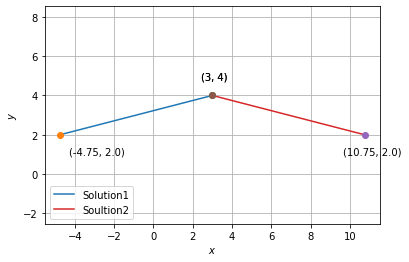
\includegraphics[width=\columnwidth]{solution.png} \label{fig:image1}
\caption{Solution}
\end{figure}
\begin{figure}[!ht]
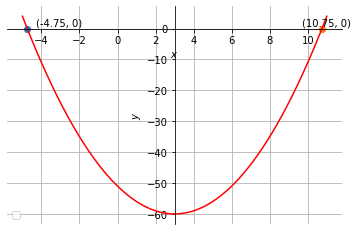
\includegraphics[width=\columnwidth]{Parabola.png} \label{fig:image1}
\caption{Quadratic equation plot}
% \label{fig2}
\end{figure}
\end{document}
